\chapter{High-pass and low-pass filters}
The main purpose of filters is to sort out unwanted frequencies from different wave-types. Filters are often used on sound files, to control the bass or the high pitch noises. There are different kinds of filters that can sort out unwanted frequencies. In this section the focus is on high and low-pass filters.

\section{Definitions}
- Here just state the different sub secs
\subsection{Low-pass filters}
The purpose of a low-pass filter is to filter out unwanted high frequencies. Listening to a such tone brings out the bass and sorts out higher pitches. The low-pass filter is in other words allowing frequencies from $0Hz$ to a chosen cut-off value. \\
The difference between a high-pass filter and a low-pass can be illustrated using a circuit diagram:
\begin{figure}[H]
	\begin{center}
\begin{circuitikz}[american voltages]
\draw (0,0)
to[sqV, sqV=$V_{AC}$] (0,2)
to (6,2)
to[short, -] (4,2)
to[C=$C$] (4,0)
to (6,0)
to (4,0)
to [resistor, R=$R$] (0,0);
\draw [>=latex', <->] (6,1.75) -- node[anchor=west] {$V_{output}$} (6,0.25);
\end{circuitikz}
\end{center}

	\caption{Circuit diagram of a low-pass filter} \label{lp:diagram}
\end{figure} 
In the illustration above the voltage output is measured around the capacitor, which decreases the high frequencies and leaves the low frequencies unchanged.  
\subsection{High-pass filters}
High-pass filters are in many ways similar to the low-pass filters. The function of the high-pass filter is straight the opposite as the low-pass filter, and its' purpose is to decrease low frequencies and leave the high frequencies unchanged. Listening to a such tone would cut off some of the base and leave the lower tones unchanged. \\
The circuit diagram for the high-pass filter is the same as the low-pass filter, but the voltage output is measured around the resistor ($R$) instead of the capacitor ($C$). This can be shown by switching around the two from figure \ref{lp:diagram}:
\begin{figure}[H]
	\begin{center}
\begin{circuitikz}[american voltages]
\draw (0,0)
to[sV, sV=$V_{AC}$] (0,2)
to (6,2)
to[short, -] (4,2)
to[resistor, R=$R$] (4,0)
to (6,0)
to (4,0)
to [C=$C$] (0,0);
\draw [>=latex', <->] (6,1.75) -- node[anchor=west] {$V_{output}$} (6,0.25);
\end{circuitikz}
\end{center}

	\caption{Circuit diagram of a high-pass filter}
\end{figure} \label{hp:diagram}
\subsection{Cut-off Frequencies}
For low-pass \\
This cut-off value can be calculated using the following equation:
\begin{align*}
f_{cutoff}=\dfrac{1}{2 \pi RC}
\end{align*}
This cut-off value describes a point on the bode plot graph, where the amplitude is decreased by $29.3\%$ and the output is decreased by $3dB$. The cut-off point is also the point, where the filtering starts getting efficient. This can be expressed using a bode plot, with the frequency on the $x-axis$ and the decibel on the $y-axis$.\\
For high-pass: \\
The high-pass filters uses the same $f_{cutoff}$ formula as the low-pass filter.

\subsection{Bode Plots}
Low-pass: \\
The $x-axis$ is a logarithmic axis, where the output is decreased by 20 decibel per decade after the cut-off point. \\
The output wave before the cut-off point will stay almost unchanged, and after the cut-off point, the amplitude is decreasing and approaching a graph that looks like a DC current. \\
High-pass: \\
When plotting the graph for the high-pass filter, the bode plot is going to be the opposite of the low-pass filters'. The graph starts in minus decibel and is approaching zero. Until it reaches the cut-off point, the graph is increasing with 20 decibel per decade. When reaching the cut-off point, the graph is 3 decibel short from reaching zero. Furthermore, $70.7\% (100\%-29.3\%)$ of the amplitude is cut off at the point $f_{cutoff}$.
\section{Derivations}
- Evt cutoff frequency ???
\section{Experiment}
- Describe experiment (purpose - what does it mean?
\subsection{Theoretical}
- How did we do in the code theoretically?
\subsection{Test Values}
- How did we get the results we did? What circuit --> refer to description after intro \\
Low-pass: \\
The bode plot looks like this:
\begin{figure}[H]
\center
	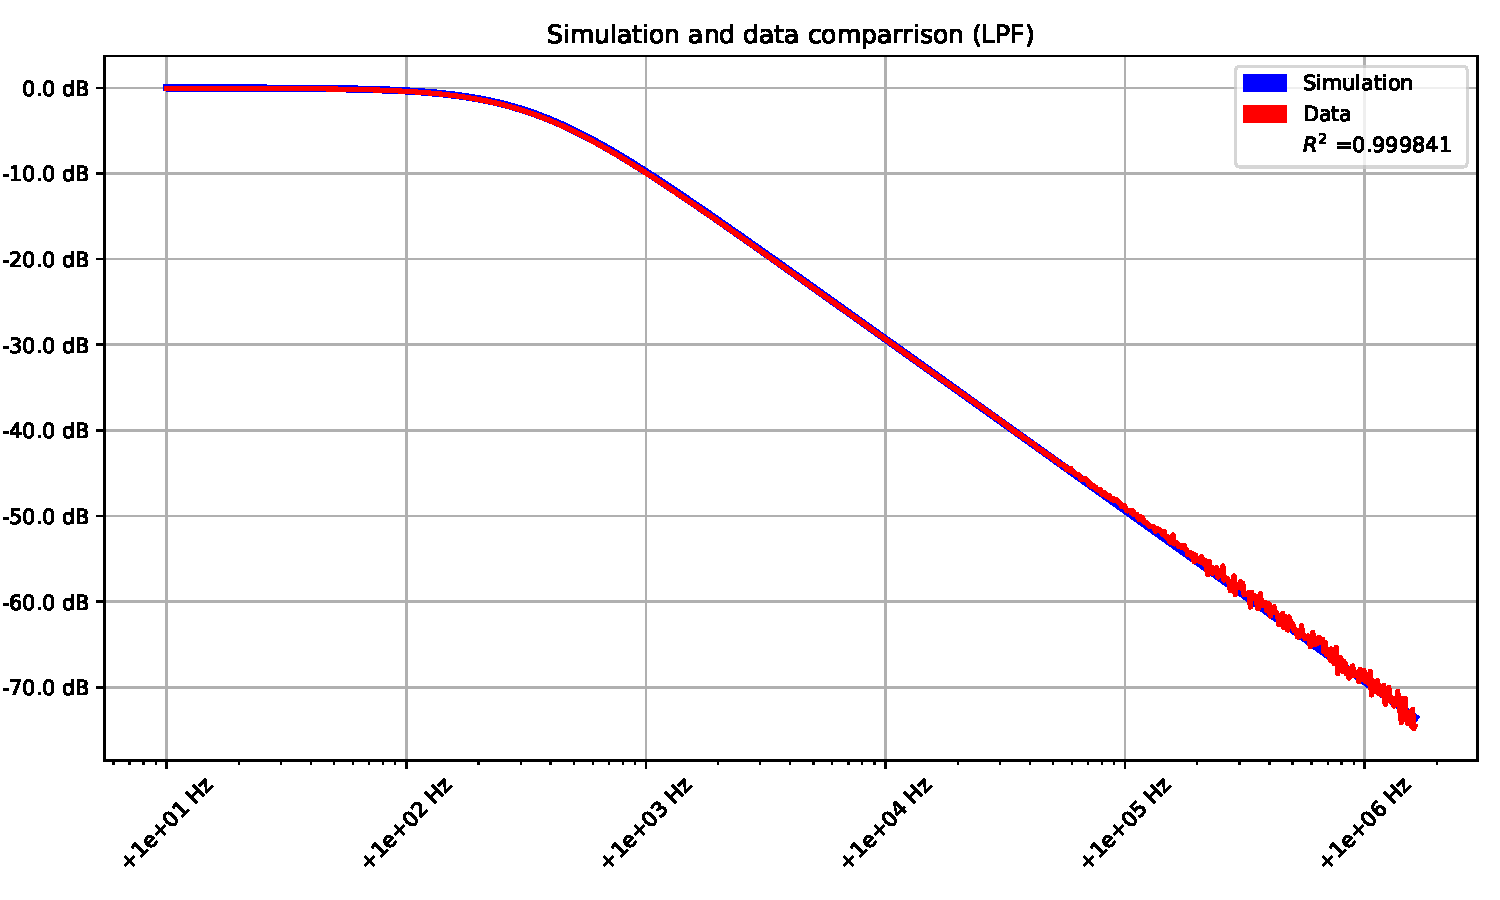
\includegraphics[scale=0.5]{fig/img/bode_LPF_plot.pdf}
	\caption{Low-pass bode plot}
	\label{lp:bode}
\end{figure}
High-pass: \\
Here is the bode plot:
\begin{figure}[H]
\center
	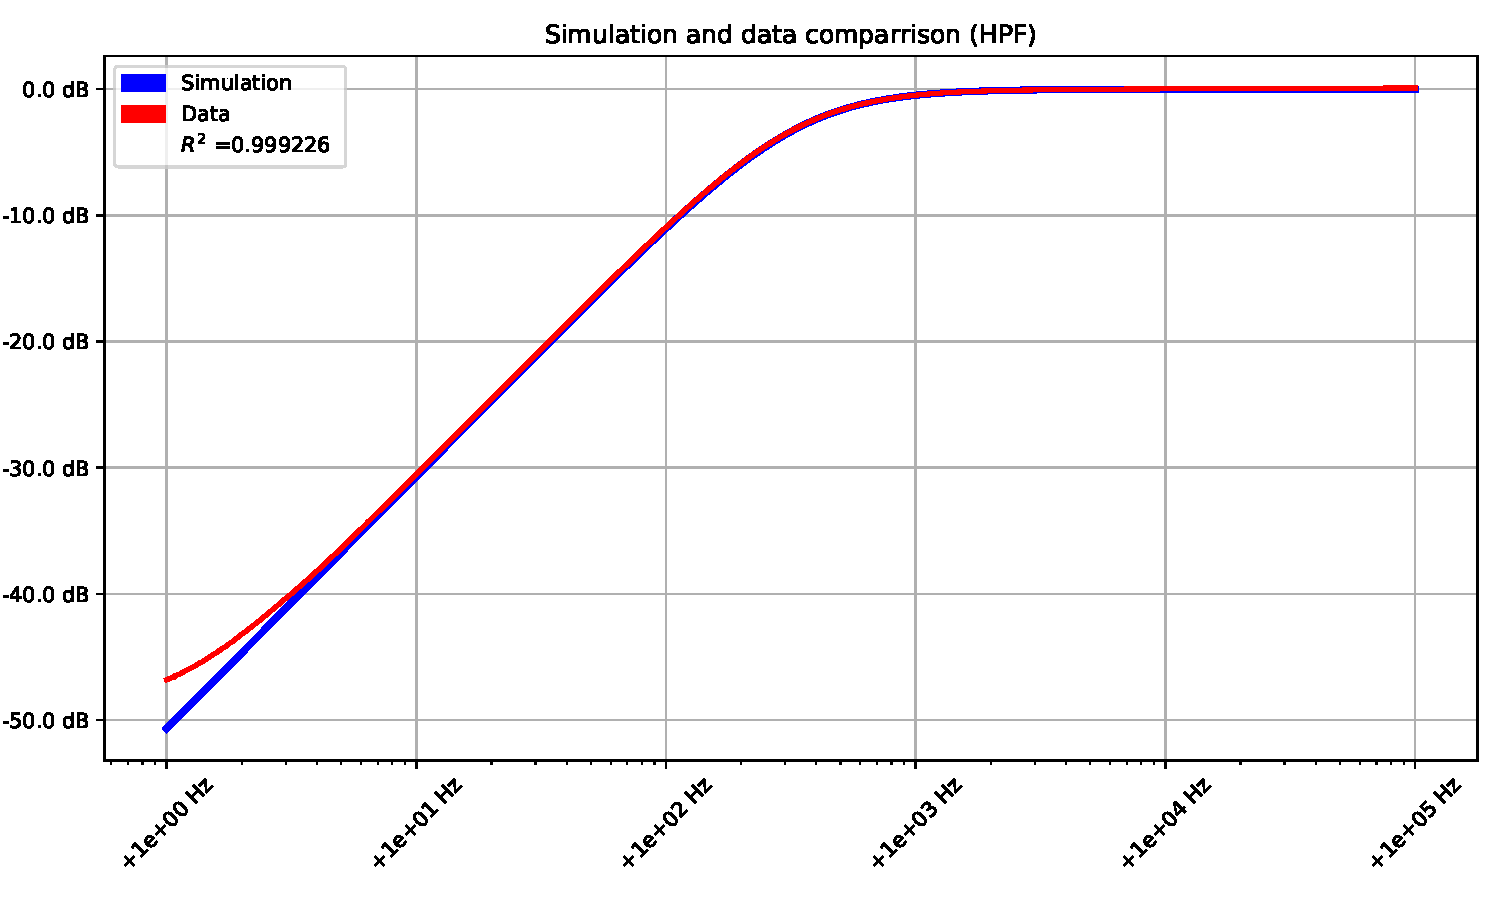
\includegraphics[scale=0.5]{fig/img/bode_HPF_plot.pdf}
	\caption{High-pass bode plot}
	\label{hp:bode}
\end{figure}
\subsection{Comparison}
- Compare the bode plots --> first low then high \\
- Describe source errors (fejlkilder) 